\documentclass{article}

\usepackage{AcademicReport}

% enable Chinese
% \usepackage[UTF8]{ctex}


% setting for levels
\usepackage{hyperref}
\setcounter{secnumdepth}{2}
\setcounter{tocdepth}{2}
\hypersetup{
    bookmarksopenlevel = 3,
    citecolor = red,
	colorlinks		=	true,
	bookmarks		=	true,
	bookmarksopen	=	true,
    % bookmarksdepth  =   2,
	pdfstartview	=	Fit,
	pdftitle		=	{PULSE LabShop Manual},
	pdfauthor		=	{Jiaxin Zhong},
}

% open book mark at arbitrary level
\usepackage[open, numbered]{bookmark}
% opt: numbered --- show numbers in the bookmark

% for some dummy text
\usepackage{lipsum}

% see https://tex.stackexchange.com/questions/226481/appendix-section-title
\usepackage[title]{appendix}


\title{\textbf{PULSE LabShop Manual}}
\author{Jiaxin Zhong}
\date{\today}

% \usepackage{mlmodern}


\begin{document}
\maketitle
% enable Page 1 of xx at the first page
\thispagestyle{firststyle}
\tableofcontents

\section{Introduction}
TBD.

Useful links:
\begin{itemize}
    \item \href{http://www.varg.unsw.edu.au/Assets/link%20pdfs/Pulse%20Labshop%20Primer%20Rev%202.pdf}{Pulse Labshop Primer} by UNSWE Vibration and Acoustics Research Group.
\end{itemize}

\section{Function analyzers}
\section{Exporting data }
\subsection{Recording files}
Steps are:
\begin{itemize}
    \item Enter \textbf{Time Data Recorder} App as shown in Fig.~\ref{fig:timedatadfjiowerfj3}.
    \item In menubar, select \textbf{Tools} $\Longrightarrow$ \textbf{Export..} as shown in Fig.~\ref{fig:fisodsexpoierj2:3902jr}.
    \item Select \textbf{mat -- MAT Files (*.mat)} as shown in Fig.~\ref{fig:fds:f0239jr0239:0wfdijf}, then click \textbf{Export}.
\end{itemize}
\begin{figure}[!htb]
    \centering
    
\includegraphics[width = 0.3\textwidth]{fig/TimeDataRecorder_20230301100611.png}
    \caption{Time Data Recorder icon}
    \label{fig:timedatadfjiowerfj3}
\end{figure}

\begin{figure}[!htb]
    \centering
    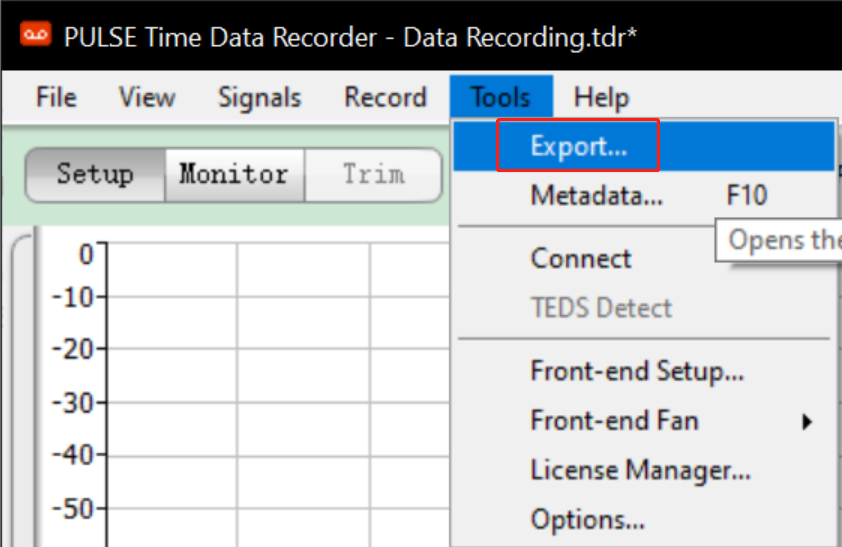
\includegraphics[width = 0.4\textwidth]{fig/Export_20230301100801.png}
    \caption{Export}
    \label{fig:fisodsexpoierj2:3902jr}
\end{figure}
\begin{figure}[!htb]
    \centering
    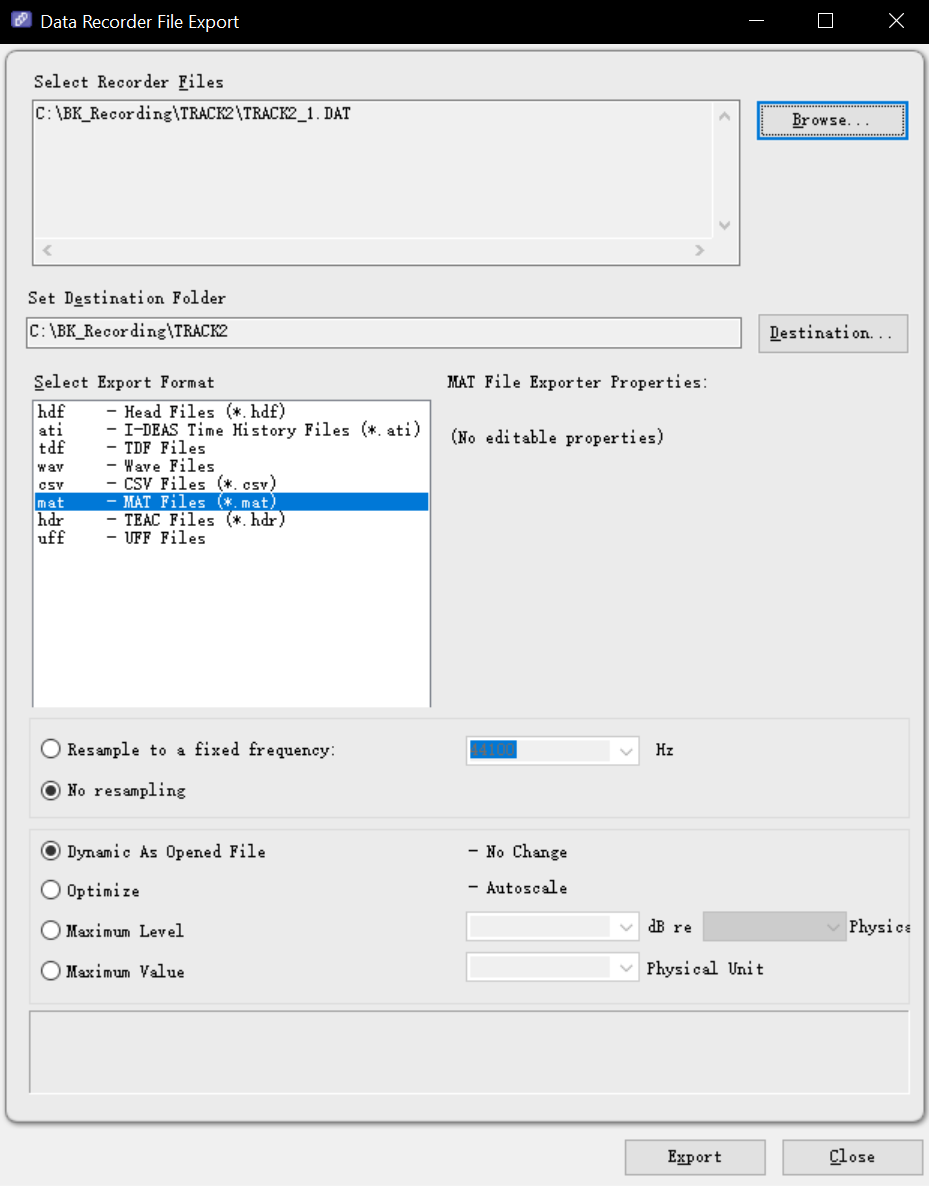
\includegraphics[width = 0.5\textwidth]{fig/DataRecorderFileExport_mat_20230301125537.png}
    \caption{Data recorder file export: .mat file.}
    \label{fig:fds:f0239jr0239:0wfdijf}
\end{figure}

As shown in Fig.~\ref{fig:fd:0392j:02w3ei2093}, select \textbf{wav -- Wave Files} to export wav files.
Make sure the resolution is \textbf{32 bit}.
\begin{figure}[!htb]
    \centering
    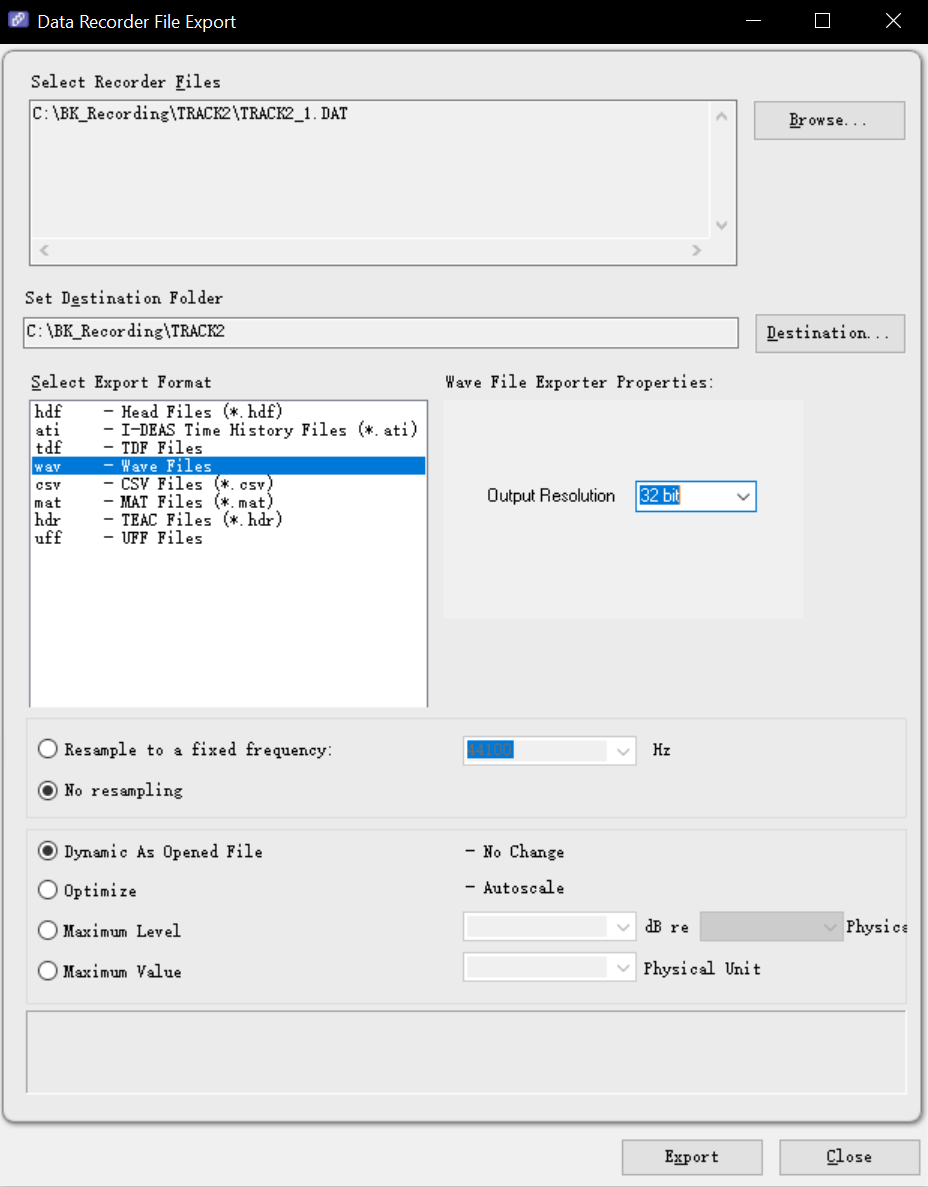
\includegraphics[width = 0.5\textwidth]{fig/DataRecorderFileExport_wav_20230301125558.png}
    \caption{Data recorder file export: .wav file.}
    \label{fig:fd:0392j:02w3ei2093}
\end{figure}




% Activate the appendix
% from now on sections are numerated with capital letters
% \begin{appendices}
% \addcontentsline{toc}{section}{Appendices}

% \section{Derivation of Eq.~(\ref{eq:29jf2})}

% \end{appendices}

\addcontentsline{toc}{section}{References}
\bibliographystyle{plain}
\bibliography{zotero}

\end{document}


